\documentclass[11pt]{article}
\usepackage[utf8]{inputenc}
\usepackage[OT1]{fontenc}
\usepackage{amsmath,amssymb}
\usepackage{graphicx}
\usepackage{booktabs}
\usepackage[margin=1in]{geometry}
\usepackage{caption}
\usepackage{natbib}
\usepackage[hidelinks,breaklinks=true]{hyperref}
\captionsetup{font=small,labelfont=bf}
\emergencystretch=2em

\title{\textbf{Quantization, Difficulty, and Item Response Theory:\\
A Proposed Framework and Pre-specified Protocol for Testing\\
When Psychometric Difficulty Signals Survive Compression}}
\author{Jung Min Kang \\[1.2ex]
Independent Researcher \\[0.4ex]
Seoul, South Korea \\[0.4ex]
\texttt{gangjeongmin23@gmail.com} \\[0.4ex]
ORCID: 0009-0007-9599-2792}
\date{\vspace{1.5\baselineskip}May 2026}

\begin{document}
\maketitle

\begin{abstract}
Quantization is evaluated almost entirely through aggregate accuracy, yet \citet{dutta2024} showed that accuracy can hide large behavioral change (``flips'') and argued that distance metrics such as KL-divergence are needed. \citet{liu2025quant} further reported that quantization-induced degradation is \emph{difficulty-dependent}: harder tasks and smaller models degrade more. This paper asks whether that difficulty dependence can be reframed as a psychometric phenomenon---a Differential Item Functioning (DIF) shift in Item Response Theory (IRT) item difficulty $b$ between precision levels---and \emph{proposes a concrete, pre-specified protocol} for testing whether such a signal is recoverable. We do not report experimental findings. Instead we contribute: (i) a framework that treats each (model, quantization-level) pair as an IRT ``subject''; (ii) five pre-specified probes, each with an explicit positive/negative decision rule, spanning difficulty recovery, accuracy-floor masking, cross-family replication, IRT-vs-averaging comparison, and the core DIF-shift test; (iii) a reference implementation (scoring, 2PL IRT fitting, KL and DIF analysis, figure generation) that runs end-to-end once response matrices are supplied; and (iv) an analysis of the regimes in which the framework is expected to be informative versus uninformative, anchored in the Evaluation Failure Scaling Law \citep{kang2026efsl}. We articulate what each probe \emph{would} show under competing hypotheses, so that the protocol can be executed at the scales where it is most likely to be diagnostic: large models, large item banks, and sparse evaluation matrices. The aim is to make the hypothesis falsifiable and the pipeline reusable, not to claim a result.
\end{abstract}

\section{Introduction}
Quantization is the dominant method for compressing large language models for deployment \citep{liu2025quant}. Nearly all quantization evaluations report aggregate accuracy on standard benchmarks; if the compressed model's accuracy is close to baseline ($\le 2$\%), the compression is deemed acceptable. \citet{dutta2024} challenged this, demonstrating that even when accuracy is preserved, a substantial fraction of individual answers can ``flip'' between correct and incorrect, and that KL-divergence captures degradation invisible to accuracy.

A separate question is whether this degradation is \emph{difficulty-dependent}. \citet{liu2025quant} report that smaller models and harder tasks degrade more under quantization. If so, this has direct implications for evaluation: simple averaging over items of mixed difficulty may systematically misestimate quantized model quality, particularly when the evaluation matrix is sparse (not all models tested on all items). The Evaluation Failure Scaling Law \citep{kang2026efsl} predicts that simple averaging collapses precisely when sparsity and difficulty gaps co-occur---the conditions under which quantization evaluation is often conducted.

We propose a psychometric reframing: treat each (model, quantization level) pair as an IRT ``subject,'' and ask whether quantization induces a measurable Differential Item Functioning \citep{holland1993} shift in item difficulty $b$ between precision groups. If the shift is difficulty-dependent (larger on harder items), then IRT-based evaluation should correct for it, while accuracy-based evaluation will not. \textbf{This paper is a proposal: we specify the framework, the probes, and the decision rules, and release a runnable reference implementation, but we do not report measured outcomes.} The contribution is a falsifiable protocol and a reusable pipeline.

\section{Proposed Framework}
\textbf{Subjects.} We propose treating each (model, quantization level) pair as an IRT subject. A representative panel that the protocol is designed for would use real GGUF weights via \texttt{llama.cpp}: e.g.\ Qwen2.5-0.5B (f16, Q8\_0, Q6\_K, Q5\_K\_M, Q4\_0, Q4\_K\_M, Q3\_K\_M, Q2\_K), Qwen2.5-1.5B (Q8\_0, Q4\_K\_M, Q2\_K), and Llama-3.2-1B (Q8\_0, Q4\_K\_M), spanning multiple effective bits-per-weight levels. A held-out model (e.g.\ Qwen2.5-3B, Q4\_K\_M) serves as an \emph{independent} external difficulty validator, never entering any panel.

\textbf{Items.} A multiple-choice benchmark such as ARC \citep{clark2018} (ARC-Easy and ARC-Challenge), scored by prompt-only next-token log-probabilities over option-letter continuations, without sampling or generation. For each item the protocol records correctness, the log-probability of the correct option, and the full option distribution (for KL). The reference implementation supplies an exact, auditable scoring routine and a response-matrix schema.

\textbf{Methods.} 2PL IRT $P(x_{ij}{=}1)=\sigma(a_j(\theta_i-b_j))$ fit by penalized MLE (L-BFGS-B, Gaussian priors), with optional masked likelihood for sparse matrices (observed cells only). KL disturbance per item is $\mathrm{KL}(\text{full}\,\|\,\text{quant})$ over the option distribution. Difficulty signals are to be validated against the independent model's per-item performance and against the benchmark's Easy/Challenge label. Primary correlation statistics would be reported with bootstrap CIs (5000 resamples) where applicable, and stability assessed with item-level cross-validation.

\section{Pre-specified Probes and Decision Rules}
We define five probes. Each states, in advance, what a positive and a negative outcome would look like, so the protocol is falsifiable rather than exploratory.

\subsection{Probe 1: Does IRT recover difficulty from quantization subjects?}
Fit a pooled 2PL over quantization-only subjects and correlate item difficulty $b$ with the external Easy/Challenge label (Spearman, AUC). \emph{Positive} if $b$ separates Easy from Challenge well above chance and is family-invariant (Qwen-only vs.\ full-panel $b$ agree) and stable under half-subject refit. \emph{Negative} if $b$ is uncorrelated with the label or unstable across refits. This probe tests whether compression preserves \emph{which items are hard}.

\subsection{Probe 2: Does accuracy mask difficulty-dependent degradation?}
On a weak model whose Challenge accuracy sits near the chance floor, accuracy cannot reveal difficulty-dependent degradation \citep{dutta2024}; the continuous KL signal may. \emph{Positive} if KL disturbance is larger on Challenge than Easy at matched compression; \emph{negative} if KL shows no difficulty dependence. A positive here is expected to be fragile and is explicitly cross-checked by Probe 3.

\subsection{Probe 3: Does any within-family effect replicate cross-family?}
Repeat the Probe-2 measurement on a different model family. \emph{Positive} only if the sign and rough magnitude replicate; \emph{negative} if a within-family effect vanishes or reverses cross-family. This guards against family-specific artifacts.

\subsection{Probe 4: Does IRT beat simple averaging as a difficulty estimator?}
Compare IRT-$b$ against item-mean accuracy for recovering the external label, in both a dense panel and a seeded sparse regime (masked-likelihood IRT vs.\ observed-cell averaging). \emph{Positive} only if IRT meaningfully exceeds averaging ($\Delta\rho$ above a pre-set margin), especially in the sparse regime; \emph{negative} if IRT merely matches averaging. The Evaluation Failure Scaling Law \citep{kang2026efsl} predicts IRT's advantage concentrates in sparse, difficulty-biased regimes, so a dense panel is expected to be uninformative for this probe.

\subsection{Probe 5: Is there a difficulty-dependent DIF shift between precision groups?}
The core test. Compute $\Delta b = b_\text{low-prec} - b_\text{high-prec}$ and correlate it with independent difficulty. \emph{Positive} if $\Delta b$ grows with difficulty (harder items shift more) with a CI excluding zero and stable cross-validated sign; \emph{negative} if $\Delta b$ is a null or sign-unstable across folds. This is the operationalization of ``quantization damages hard items more,'' expressed as psychometric DIF.

\begin{figure}[t]
\centering
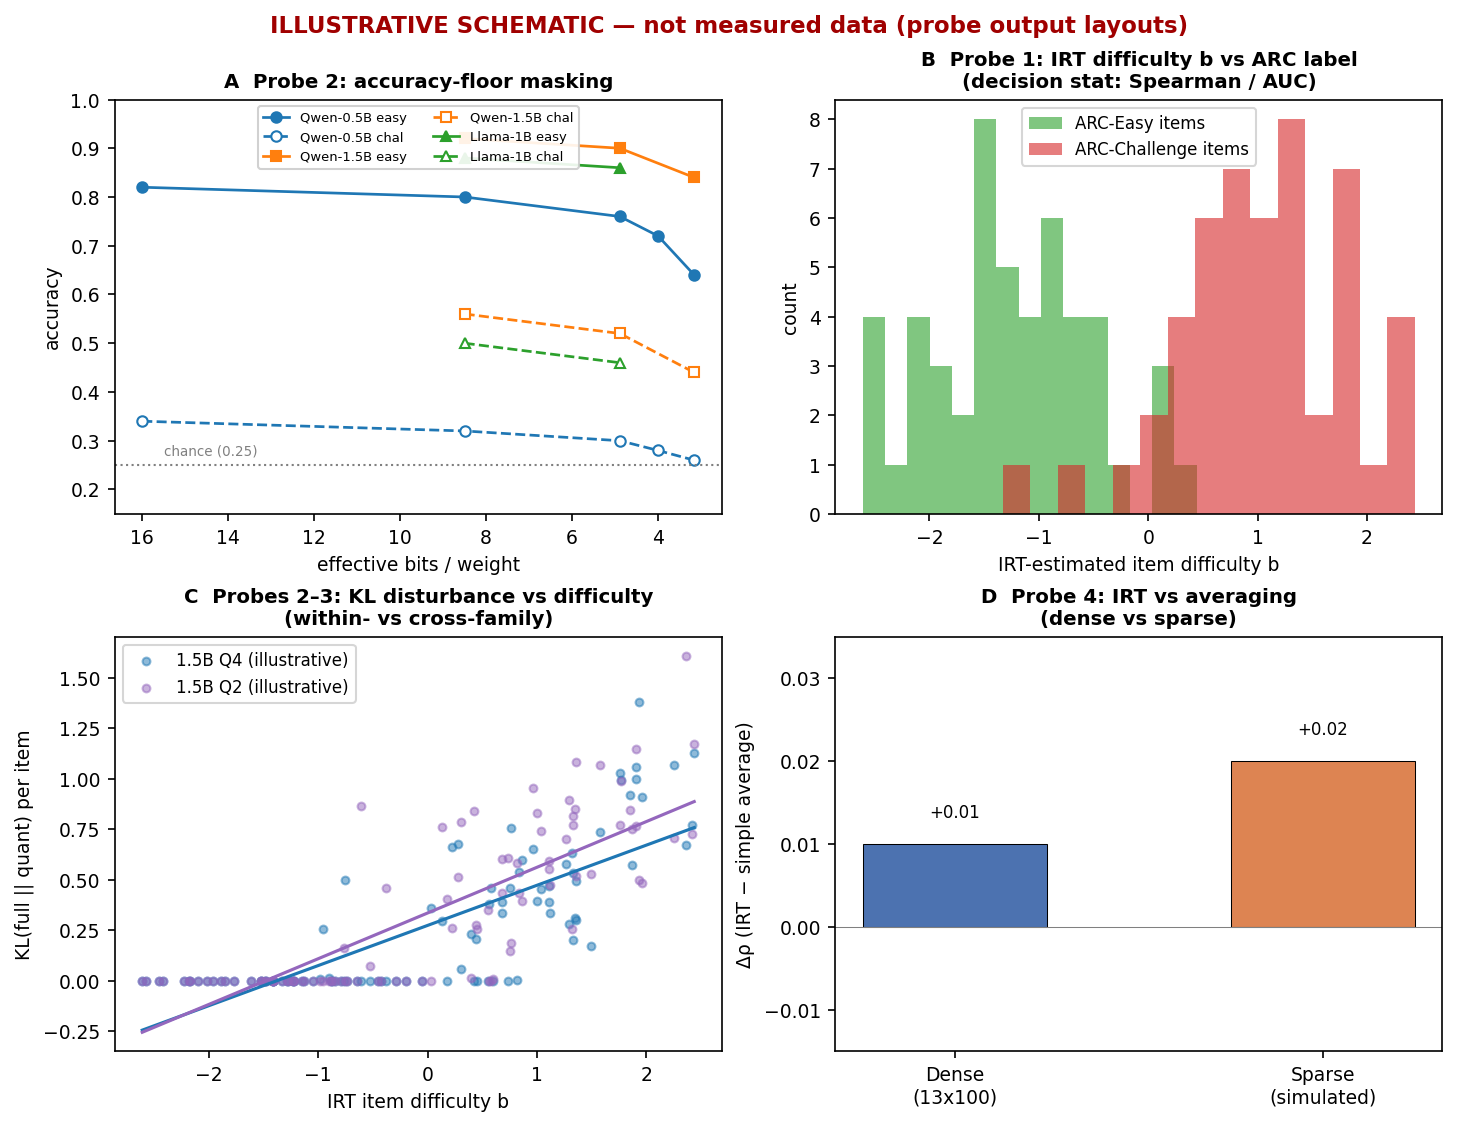
\includegraphics[width=\textwidth]{figures/fig1_main.png}
\caption{\textbf{Illustrative schematic (not measured data).} Mock layouts showing the \emph{form} each probe's output would take. \textbf{A:} accuracy-floor view (Probe 2): a weak model's Challenge accuracy near the chance floor would mask degradation that KL could still expose. \textbf{B:} difficulty-recovery view (Probe 1): the distribution of IRT $b$ for Easy vs.\ Challenge items. \textbf{C:} KL-vs-difficulty view (Probes 2--3): within- vs.\ cross-family relationships. \textbf{D:} IRT-vs-averaging view (Probe 4): $\Delta\rho$ in dense vs.\ sparse regimes. Values shown are placeholders illustrating axes and layout only; they are not experimental results.}
\label{fig:main}
\end{figure}

\begin{figure}[t]
\centering
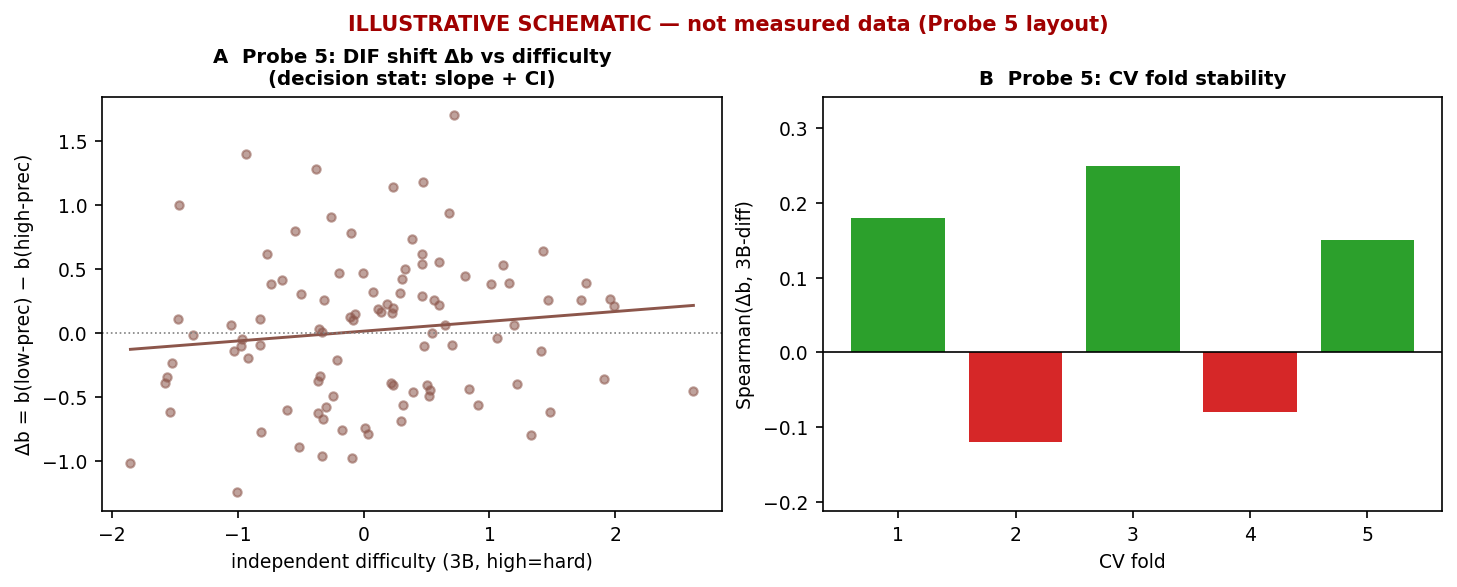
\includegraphics[width=0.92\textwidth]{figures/fig2_dif.png}
\caption{\textbf{Illustrative schematic (not measured data).} The form of the Probe-5 output. \textbf{A:} the DIF shift $\Delta b$ plotted against independent difficulty, with the regression slope and CI as the decision statistic. \textbf{B:} cross-validation fold stability, where sign-flipping across folds would indicate a null. Points are placeholders demonstrating the intended visualization, not findings.}
\label{fig:dif}
\end{figure}

\section{Expected Regimes of Informativeness}
The framework is most likely to be diagnostic where psychometric modeling is known to help and least likely where simple statistics already suffice. Following the Evaluation Failure Scaling Law \citep{kang2026efsl}, IRT's advantage over averaging is expected to concentrate in \emph{sparse, difficulty-biased} matrices. A dense small panel (few models, fully crossed with few items) sits in the region where averaging is already near-optimal, so Probe 4 is expected to be uninformative there; Probe 5 likewise demands large item banks to estimate $\Delta b$ with usable precision. Prior work establishes difficulty-dependent degradation at substantial scale---\citet{liu2025quant} span 1.5B--70B models on full reasoning benchmarks and \citet{dutta2024} go up to 70B---so we expect the protocol to be most informative when executed with large models, large item banks, and deliberately sparsified evaluation matrices, and we make those the recommended operating points.

\section{Reference Implementation}
We release a runnable pipeline implementing the framework end-to-end: \texttt{run\_eval.py} (prompt-only next-token option scoring with tokenizer diagnostics), \texttt{analyze\_all.py} (2PL IRT with optional masked likelihood, KL, DIF, bootstrap CIs, cross-validation, and a seeded sparse simulation), and \texttt{make\_figs.py} (which plots real per-item data when response matrices are present and otherwise renders clearly-labeled illustrative schematics). A manifest checker verifies that all required inputs are present before analysis. The package includes the response-matrix schema and an example findings file documenting the output format. Supplying a panel of scored response matrices reproduces every probe statistic and replaces the illustrative figures with measured ones.

\section{Limitations and Scope}
This is a proposal: it contributes a framework, a falsifiable protocol, and a reference implementation, and it deliberately makes \emph{no} empirical claim about any specific model or quantization scheme. The figures are illustrative schematics, not measurements. The protocol's own expected weak points are stated in advance: single-benchmark scoring, greedy decoding without per-item variance, weight-only GGUF K-quantization (IQ-quant and activation quantization out of scope), and reliance on a model-based external difficulty validator rather than human calibration. Effective bits-per-weight, where displayed, follow the canonical \texttt{llama.cpp} reference table (Llama-3.1-8B) and vary by architecture. Whether the difficulty-dependent DIF shift exists is left as the open empirical question the protocol is designed to answer.

\section{Conclusion}
We have reframed difficulty-dependent quantization degradation as a question about Item Response Theory difficulty, and turned it into a falsifiable, pre-specified protocol with explicit decision rules and a reusable reference implementation. We do not claim to have shown that compression preserves item difficulty, nor that a DIF shift does or does not exist; we specify exactly how to find out. The framework is offered so that others can execute it at the scales where it is most likely to be diagnostic---large models, large item banks, and sparse evaluation matrices---and report what they find.

\paragraph{Code availability.} A reference implementation (\texttt{run\_eval.py}, \texttt{analyze\_all.py}, \texttt{make\_figs.py}, \texttt{scripts/check\_manifest.py}), the response-matrix schema, and an example findings file documenting output format are released as a code repository. The figures in this paper are illustrative schematics generated by that code in the absence of measured response matrices; supplying real matrices reproduces every probe and replaces the schematics with measured results.\\ Code: \url{https://github.com/testofschool/irt-quantization}.

\begin{thebibliography}{9}
\bibitem[Dutta et al.(2024)]{dutta2024} A.~Dutta, S.~Krishnan, N.~Kwatra, and R.~Ramjee. Accuracy is Not All You Need. \emph{NeurIPS}, 2024. arXiv:2407.09141.
\bibitem[Liu et al.(2025)]{liu2025quant} R.~Liu, Y.~Sun, M.~Zhang, H.~Bai, X.~Yu, T.~Yu, C.~Yuan, and L.~Hou. Quantization Hurts Reasoning? An Empirical Study on Quantized Reasoning Models. \emph{COLM}, 2025. arXiv:2504.04823.
\bibitem[Holland \& Wainer(1993)]{holland1993} P.~W.~Holland and H.~Wainer. \emph{Differential Item Functioning}. Lawrence Erlbaum, 1993.
\bibitem[Kang(2026)]{kang2026efsl} J.~M.~Kang. The Scaling Law of Evaluation Failure. arXiv:2605.11205, 2026.
\bibitem[Clark et al.(2018)]{clark2018} P.~Clark, I.~Cowhey, O.~Etzioni, T.~Khot, A.~Sabharwal, C.~Schoenick, and O.~Tafjord. Think you have Solved Question Answering? Try ARC, the AI2 Reasoning Challenge. arXiv:1803.05457, 2018.
\end{thebibliography}

\end{document}
